% =========================================================================== %
% One Day Tutorial
% =========================================================================== %

\ifx\wholebook\relax\else
  \documentclass[a4paper,10pt,twoside]{book}
  %=============================================================================%
% Common things, settings, packages to include
%=============================================================================%

\usepackage{graphicx}
\usepackage{color}
\usepackage{makeidx}
\usepackage{ifpdf}
\usepackage{verbatim}

% --------------------------------------------------------------------------- %
% Setting up stuff depeding on output format
% --------------------------------------------------------------------------- %

\ifpdf
  % special settings for pdf mode
  \usepackage[colorlinks]{hyperref}
  \usepackage{courier}
  
  \hypersetup{
    colorlinks,
    linkcolor=darkblue,
    citecolor=darkblue,
    pdftitle={The Eclipse Scout Book},
    pdfauthor={The Scout Community},
    pdfkeywords={Enterprise Framework, Eclipse, Java, Client-Side, Rich Client, Web Client, Mobile},
    pdfsubject={Computer Science}
  }
  
  \usepackage{caption}
  \captionsetup{margin=10pt,font=small,labelfont=bf}
\else
  % special stuff for html mode
  \usepackage[tex4ht]{hyperref}
\fi

% --------------------------------------------------------------------------- %
% Setting up printing range
% --------------------------------------------------------------------------- %

\parindent 1cm
\parskip 0.2cm
\topmargin 0.2cm
\oddsidemargin 1cm
\evensidemargin 0.5cm
\textwidth 15cm
\textheight 21cm

% --------------------------------------------------------------------------- %
% Setting up listings
% --------------------------------------------------------------------------- %

\usepackage{listings}
 
\definecolor{darkviolet}{rgb}{0.5,0,0.4}
\definecolor{darkgreen}{rgb}{0,0.4,0.2} 
\definecolor{darkblue}{rgb}{0.1,0.1,0.9}
\definecolor{darkgrey}{rgb}{0.5,0.5,0.5}
\definecolor{lightblue}{rgb}{0.4,0.4,1}
\definecolor{lightgray}{rgb}{0.97,0.97,0.97}

\renewcommand{\lstlistlistingname}{List of Listings}

% general settings
\lstset{
  basicstyle=\small\ttfamily,
  columns=fullflexible,
  breaklines=true,
  breakindent=10pt,
  prebreak=\mbox{{\color{blue}\tiny$\searrow$}},
  postbreak=\mbox{{\color{blue}\tiny$\rightarrow$}},
  showstringspaces=false,
  backgroundcolor=\color{lightgray}
}

% settings for xml files
\lstdefinelanguage{xml}
{
  commentstyle=\color{darkgrey}\upshape,
  morestring=[b]",
  morestring=[s]{>}{<},
  morecomment=[s]{<?}{?>},
  stringstyle=\color{black},
  identifierstyle=\color{darkblue},
  keywordstyle=\color{cyan},
  morekeywords={xmlns,name,point,factory,class}% list your attributes here
}

% settings for ini files
\lstdefinelanguage{ini}
{
  morecomment=[f][\color{darkgrey}\upshape][0]\#, % # is comment iff it's the first char on the line
  stringstyle=\color{black}
}

% default settings (for java files)
\lstset{
  language=Java,
  emphstyle=\color{red}\bfseries,
  keywordstyle=\color{darkviolet}\bfseries,
  commentstyle=\color{darkgreen},
  morecomment=[s][\color{lightblue}]{/**}{*/},
  stringstyle=\color{darkblue},
}

% --------------------------------------------------------------------------- %
% cross reference macros
% --------------------------------------------------------------------------- %
\newcommand{\applabel}[1]{\label{apx:#1}}
\newcommand{\chalabel}[1]{\label{cha:#1}}
\newcommand{\seclabel}[1]{\label{sec:#1}}
\newcommand{\lstlabel}[1]{\label{lst:#1}}
\newcommand{\figlabel}[1]{\label{fig:#1}}
\newcommand{\tablabel}[1]{\label{tab:#1}}

\newcommand{\appref}[1]{Appendix~\ref{apx:#1}}
\newcommand{\charef}[1]{Chapter~\ref{cha:#1}\xspace}
\newcommand{\secref}[1]{Section~\ref{sec:#1}}
\newcommand{\lstref}[1]{Listing~\ref{lst:#1}\xspace}
\newcommand{\figref}[1]{Figure~\ref{fig:#1}\xspace}
\newcommand{\tabref}[1]{Table~\ref{tab:#1}\xspace}

% --------------------------------------------------------------------------- %
% graphics paths
% --------------------------------------------------------------------------- %
\graphicspath{
  {figures/}
  {Introduction/figures/}
}

%=============================================================================%

  \pagestyle{headings}
  \graphicspath{{figures/} {../figures/}}
  \begin{document}
  \sloppy
\fi

% --------------------------------------------------------------------------- %
\chapter{A Larger Example}
\chalabel{large_example}

In this chapter we will create a small Scout application that covers additional aspects of the Eclipse Scout framework. 
Specifically, we will build an outline based Scout application featuring a navigation tree and pages to present information in tabular form. 
In addition, the application also shows how to work with menus and context menus, search forms, and forms to enter and/or update data. 
On the server side we show how to work with databases, how to use logging in Scout applications and how to include standard Java libraries. 

This chapter is organized as follows.
First, the finished demo application is explained from the user perspective.
Then bla.
\footnote{
Social networking services according to Wikipedia: \url{http://en.wikipedia.org/wiki/Social_network_service}
}

% --------------------------------------------------------------------------- %
\section{The "My Contacts" Application}

\noindent Existing Documentation
\begin{itemize}
  \item minicrm tutorial \url{http://wiki.eclipse.org/Scout/Tutorial/3.8/Minicrm/Minicrm_Step-by-Step}
  \item permissions/roles wiki tutorial \url{http://wiki.eclipse.org/Scout/Tutorial/3.8/Minicrm/Permissions}
\end{itemize}

same pointer in scout server, security, and one day tutorial

\section{The Implementation}

new scout project \java{org.eclipsescout.contacts}, tree and table (outline based app)

\begin{figure}
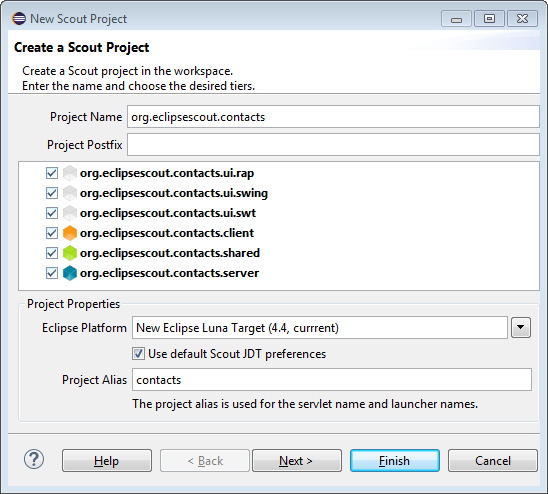
\includegraphics[width=7cm]{new_project_contacts_1.png} \hspace{5mm}
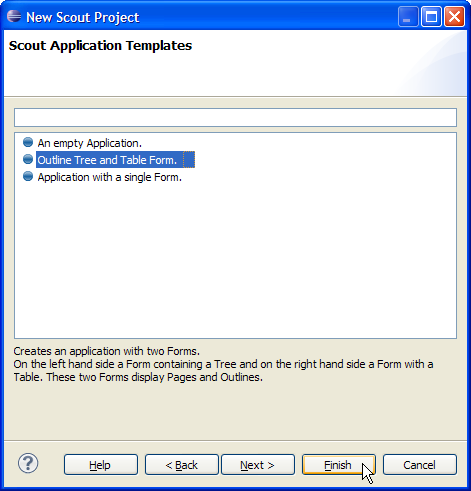
\includegraphics[width=7cm]{new_project_contacts_2.png}
\caption{Start with creating a new Scout project. }
\figlabel{new_project_contacts_1}
\end{figure}

Lorem ipsum will build an outline based Scout application featuring a navigation tree and pages to present information in tabular form. 
In addition, the application also shows how to work with menus and context menus, search forms, and forms to enter and/or update data. 
On the server side we show how to work with databases, how to use logging in Scout applications and how to lorem ipsum. 

\begin{figure}
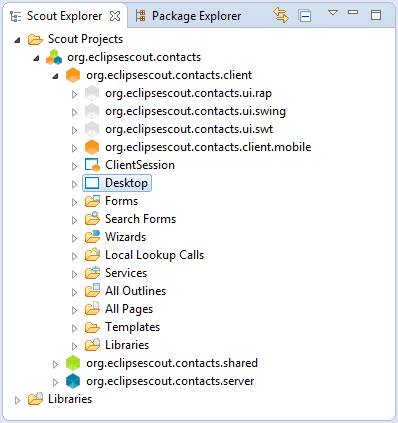
\includegraphics[width=7cm]{desktop_explorer.png} \hspace{5mm}
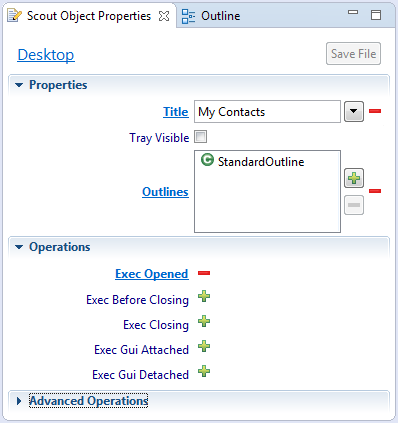
\includegraphics[width=7cm]{desktop_properties.png}
\caption{Configure the application name in the \field{Title} of the Desktop's properties. }
\figlabel{new_project_contacts_1}
\end{figure}

Lorem ipsum will build an outline based Scout application featuring a navigation tree and pages to present information in tabular form. 
In addition, the application also shows how to work with menus and context menus, search forms, and forms to enter and/or update data. 
On the server side we show how to work with databases, how to use logging in Scout applications and how to lorem ipsum. 

\begin{figure}
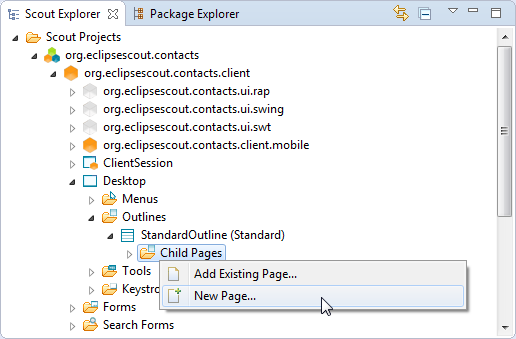
\includegraphics[width=5cm]{new_page_person_contextmenu.png} \hspace{2mm}
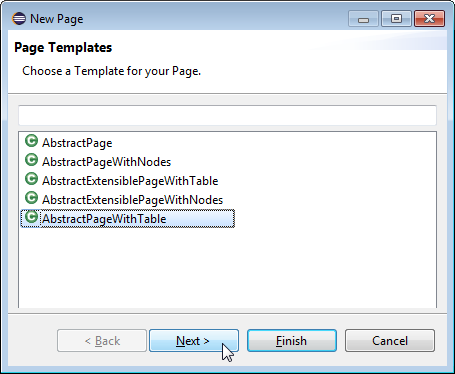
\includegraphics[width=4.5cm]{new_page_person_1.png} \hspace{2mm}
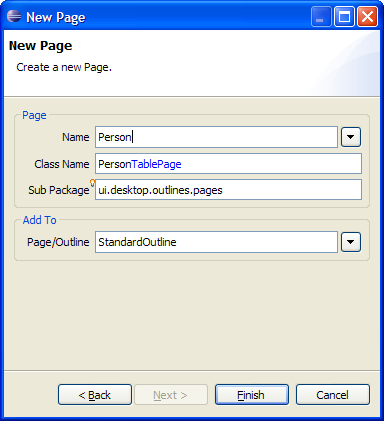
\includegraphics[width=4.5cm]{new_page_person_2.png}
\caption{Add the person table page below the standard outline. }
\figlabel{new_page_person}
\end{figure}

Lorem ipsum will build an outline based Scout application featuring a navigation tree and pages to present information in tabular form. 
In addition, the application also shows how to work with menus and context menus, search forms, and forms to enter and/or update data. 
On the server side we show how to work with databases, how to use logging in Scout applications and how to lorem ipsum. 

\begin{figure}
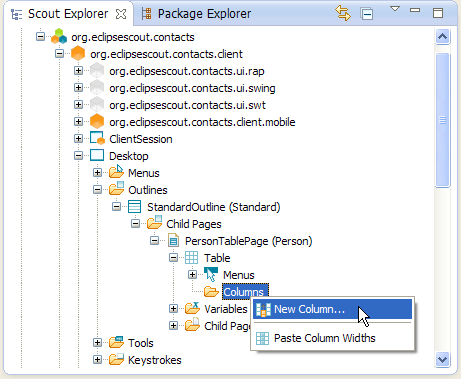
\includegraphics[width=5cm]{new_column_personid_contextmenu.png} \hspace{2mm}
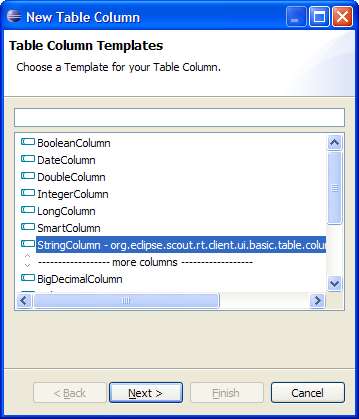
\includegraphics[width=4.5cm]{new_column_personid_1.png} \hspace{2mm}
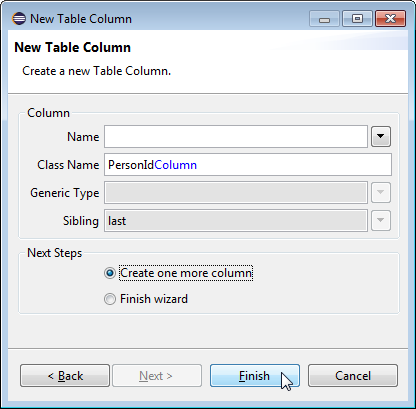
\includegraphics[width=4.5cm]{new_column_personid_2.png}
\caption{Add columns to the person page. }
\figlabel{new_column_personid}
\end{figure}

Lorem ipsum will build an outline based Scout application featuring a navigation tree and pages to present information in tabular form. 
In addition, the application also shows how to work with menus and context menus, search forms, and forms to enter and/or update data. 
On the server side we show how to work with databases, how to use logging in Scout applications and how to lorem ipsum. 

\begin{figure}
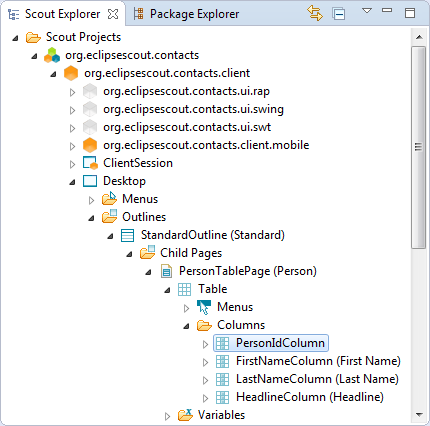
\includegraphics[height=7cm]{person_id_column.png} \hspace{5mm}
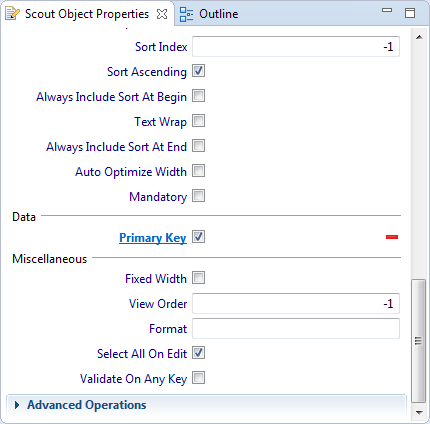
\includegraphics[height=7cm]{person_id_property.png}
\caption{Configure the \element{PersonId} column. Check property \element{Primary Key} under the section \elment{Advanced Properties} (right).}
\figlabel{new_column_personid}
\end{figure}

Lorem ipsum will build an outline based Scout application featuring a navigation tree and pages to present information in tabular form. 
In addition, the application also shows how to work with menus and context menus, search forms, and forms to enter and/or update data. 
On the server side we show how to work with databases, how to use logging in Scout applications and how to lorem ipsum. 

\begin{figure}
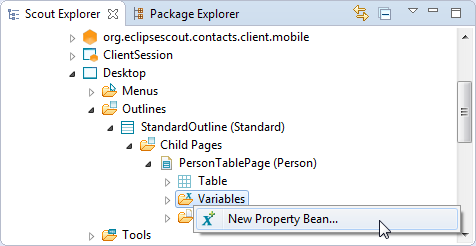
\includegraphics[height=5cm]{new_bean_companyid_contextmenu.png} \hspace{5mm}
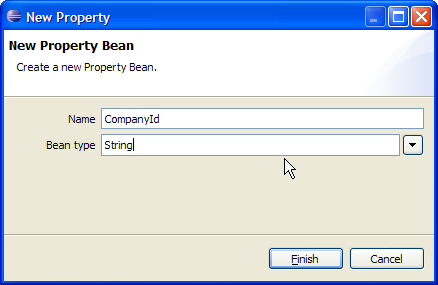
\includegraphics[height=5cm]{new_bean_companyid.png}
\caption{Add the \element{CompanyId} variable to the person page.}
\figlabel{new_bean_companyid}
\end{figure}

Lorem ipsum will build an outline based Scout application featuring a navigation tree and pages to present information in tabular form. 
In addition, the application also shows how to work with menus and context menus, search forms, and forms to enter and/or update data. 
On the server side we show how to work with databases, how to use logging in Scout applications and how to lorem ipsum. 

\begin{figure}
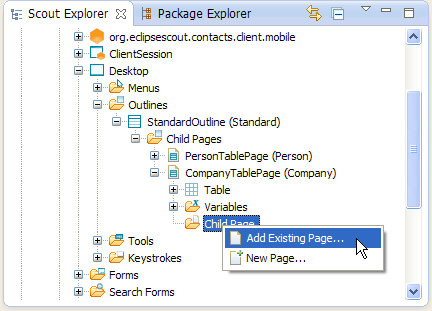
\includegraphics[width=6.5cm]{add_existing_page_contextmenu.png} \hspace{5mm}
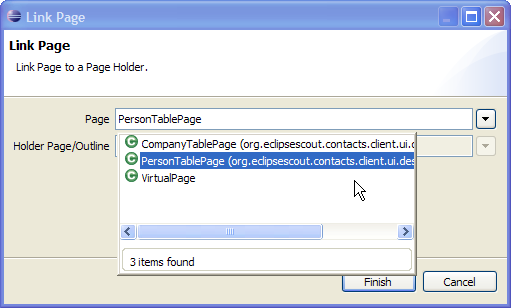
\includegraphics[width=7.5cm]{add_existing_page.png}
\caption{Add the person page below the the company page.}
\figlabel{add_existing_page}
\end{figure}

Lorem ipsum will build an outline based Scout application featuring a navigation tree and pages to present information in tabular form. 
In addition, the application also shows how to work with menus and context menus, search forms, and forms to enter and/or update data. 
On the server side we show how to work with databases, how to use logging in Scout applications and how to lorem ipsum. 

\begin{figure}
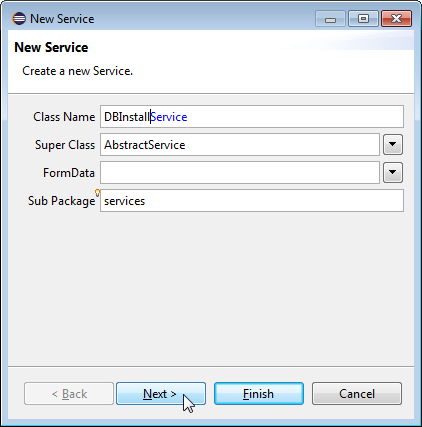
\includegraphics[width=7cm]{new_service_dbinstall_1.png} \hspace{5mm}
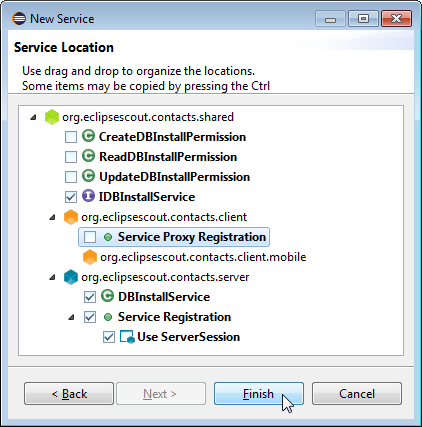
\includegraphics[width=7cm]{new_service_dbinstall_2.png} 
\caption{Add a database installation service. }
\figlabel{new_service_dbinstall}
\end{figure}

Lorem ipsum will build an outline based Scout application featuring a navigation tree and pages to present information in tabular form. 
In addition, the application also shows how to work with menus and context menus, search forms, and forms to enter and/or update data. 
On the server side we show how to work with databases, how to use logging in Scout applications and how to lorem ipsum. 

\begin{figure}
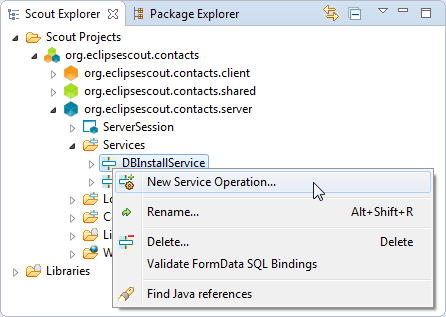
\includegraphics[height=5.5cm]{new_operation_installstorage_contextmenu.png} \hspace{5mm}
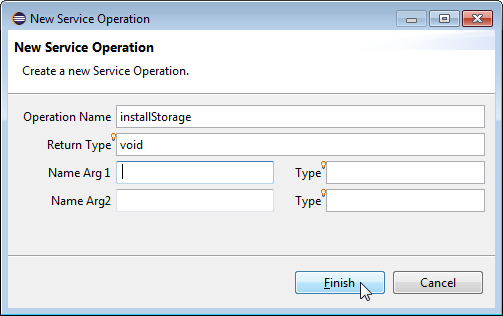
\includegraphics[height=5.5cm]{new_operation_installstorage.png} 
\caption{Add the service operation to create the DB schema. }
\figlabel{new_operation_installstorage}
\end{figure}

Lorem ipsum will build an outline based Scout application featuring a navigation tree and pages to present information in tabular form. 
In addition, the application also shows how to work with menus and context menus, search forms, and forms to enter and/or update data. 
On the server side we show how to work with databases, how to use logging in Scout applications and how to lorem ipsum. 

\begin{figure}
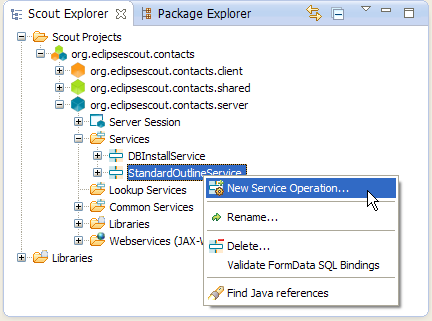
\includegraphics[height=5.5cm]{new_service_persontabledata_contextmenu.png} \hspace{5mm}
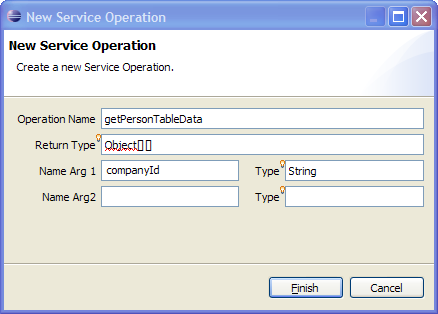
\includegraphics[height=5.5cm]{new_service_persontabledata.png}
\caption{Add the service operation to fetch the data for the person table. }
\figlabel{new_service_persontabledata}
\end{figure}

Lorem ipsum will build an outline based Scout application featuring a navigation tree and pages to present information in tabular form. 
In addition, the application also shows how to work with menus and context menus, search forms, and forms to enter and/or update data. 
On the server side we show how to work with databases, how to use logging in Scout applications and how to lorem ipsum. 

\begin{figure}
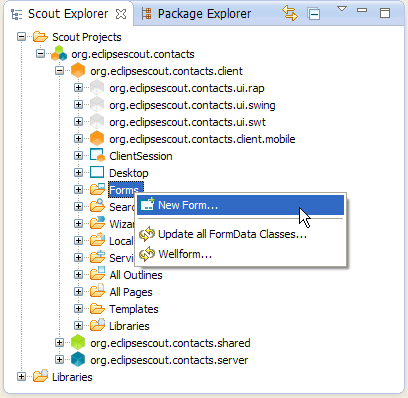
\includegraphics[height=7cm]{new_form_person_contextmenu.png} \hspace{5mm}
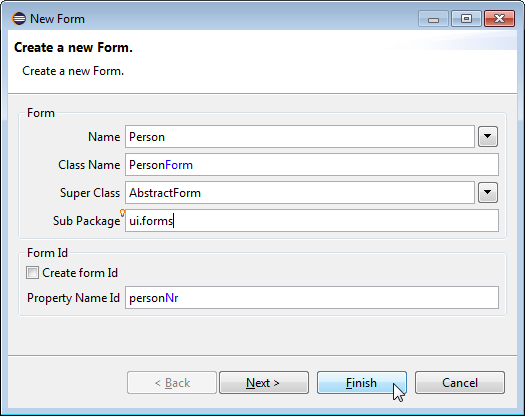
\includegraphics[height=7cm]{new_form_person.png}
\caption{Add the person form.}
\figlabel{new_form_person}
\end{figure}

Lorem ipsum will build an outline based Scout application featuring a navigation tree and pages to present information in tabular form. 
In addition, the application also shows how to work with menus and context menus, search forms, and forms to enter and/or update data. 
On the server side we show how to work with databases, how to use logging in Scout applications and how to lorem ipsum. 

\begin{figure}
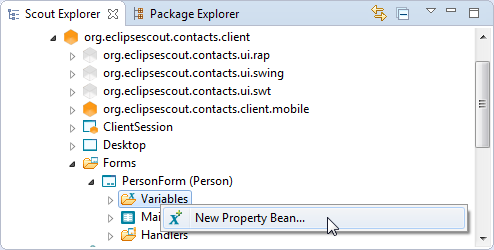
\includegraphics[height=5cm]{new_bean_personid_contextmenu.png} \hspace{5mm}
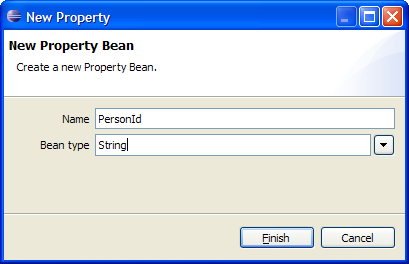
\includegraphics[height=5cm]{new_bean_personid.png}
\caption{Add the \element{PersonId} variable to the person form.}
\figlabel{new_bean_personid}
\end{figure}

Lorem ipsum will build an outline based Scout application featuring a navigation tree and pages to present information in tabular form. 
In addition, the application also shows how to work with menus and context menus, search forms, and forms to enter and/or update data. 
On the server side we show how to work with databases, how to use logging in Scout applications and how to lorem ipsum. 

\begin{figure}
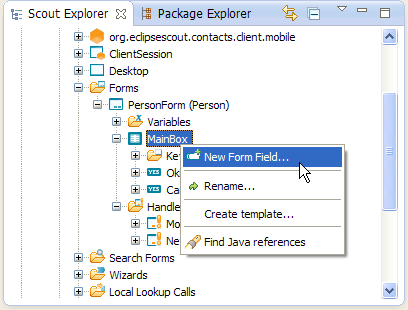
\includegraphics[width=7cm]{new_field_personbox.png} \hspace{5mm}
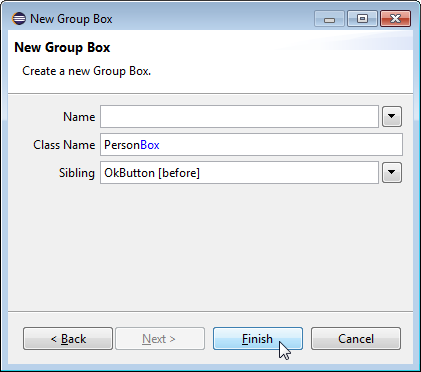
\includegraphics[width=7cm]{new_field_personbox_name.png}
\caption{Add the first group box field to the person form.}
\figlabel{new_field_personbox}
\end{figure}

Lorem ipsum will build an outline based Scout application featuring a navigation tree and pages to present information in tabular form. 
In addition, the application also shows how to work with menus and context menus, search forms, and forms to enter and/or update data. 
On the server side we show how to work with databases, how to use logging in Scout applications and how to lorem ipsum. 

\begin{figure}
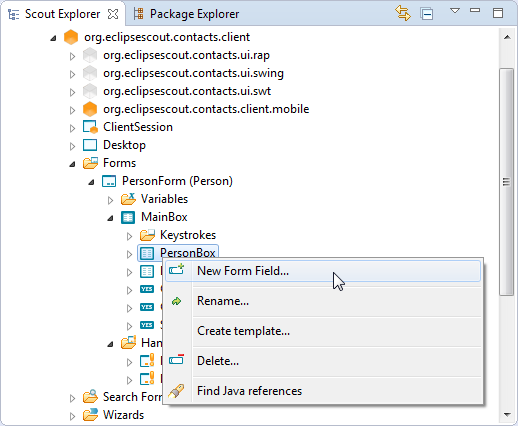
\includegraphics[width=7cm]{new_field_picture_contextmenu.png} \hspace{5mm}
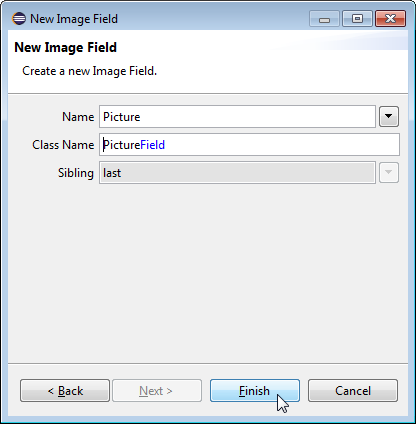
\includegraphics[width=7cm]{new_field_picture.png}
\caption{Add the picture field to the first group box of the person form.}
\figlabel{new_field_picture}
\end{figure}

Lorem ipsum will build an outline based Scout application featuring a navigation tree and pages to present information in tabular form. 
In addition, the application also shows how to work with menus and context menus, search forms, and forms to enter and/or update data. 
On the server side we show how to work with databases, how to use logging in Scout applications and how to lorem ipsum. 

\begin{figure}
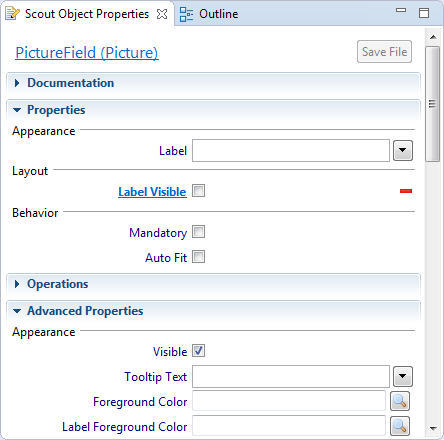
\includegraphics[width=7cm]{picture_field_properties_1.png} \hspace{5mm}
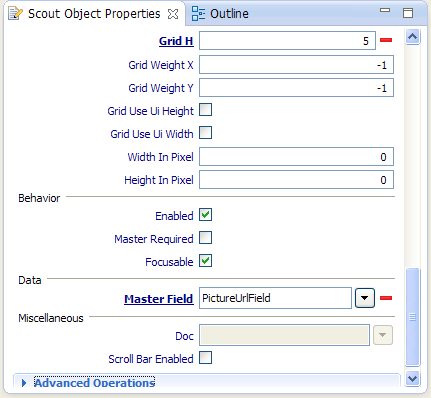
\includegraphics[width=7cm]{picture_field_properties_2.png}
\caption{Set the properties for the picture field of the person form.}
\figlabel{picture_field_properties}
\end{figure}

Lorem ipsum will build an outline based Scout application featuring a navigation tree and pages to present information in tabular form. 
In addition, the application also shows how to work with menus and context menus, search forms, and forms to enter and/or update data. 
On the server side we show how to work with databases, how to use logging in Scout applications and how to lorem ipsum. 

\begin{figure}
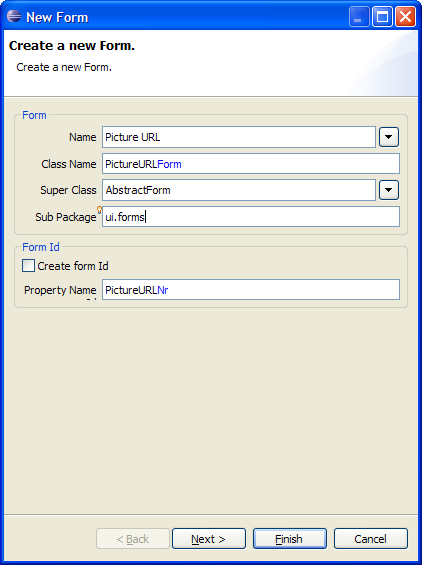
\includegraphics[width=7cm]{new_form_url_1.png} \hspace{5mm}
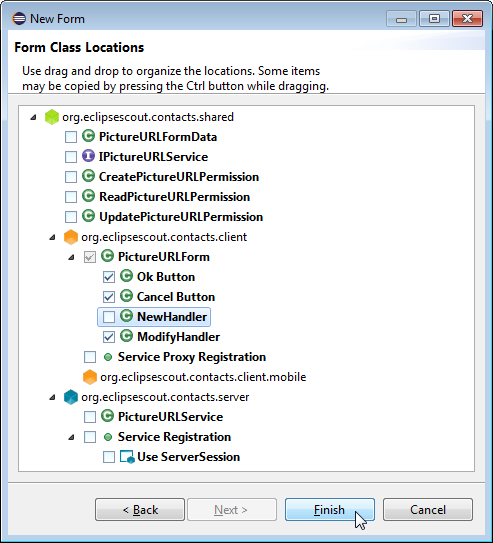
\includegraphics[width=7cm]{new_form_url_2.png}
\caption{Add the URL editor form.}
\figlabel{new_form_url}
\end{figure}

Lorem ipsum will build an outline based Scout application featuring a navigation tree and pages to present information in tabular form. 
In addition, the application also shows how to work with menus and context menus, search forms, and forms to enter and/or update data. 
On the server side we show how to work with databases, how to use logging in Scout applications and how to lorem ipsum. 

\begin{figure}
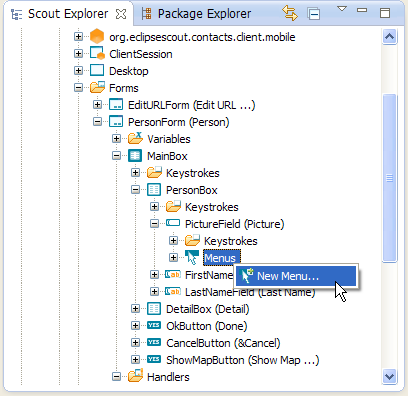
\includegraphics[width=7cm]{new_menu_editurl_contextmenu.png} \hspace{5mm}
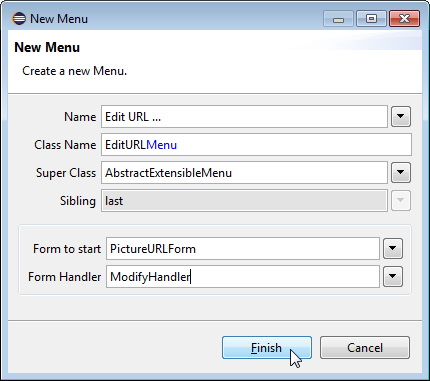
\includegraphics[width=7cm]{new_menu_editurl.png}
\caption{Add the URL edit menu to the picture field.}
\figlabel{new_menu_editurl}
\end{figure}

Lorem ipsum will build an outline based Scout application featuring a navigation tree and pages to present information in tabular form. 
In addition, the application also shows how to work with menus and context menus, search forms, and forms to enter and/or update data. 
On the server side we show how to work with databases, how to use logging in Scout applications and how to lorem ipsum. 

\begin{figure}
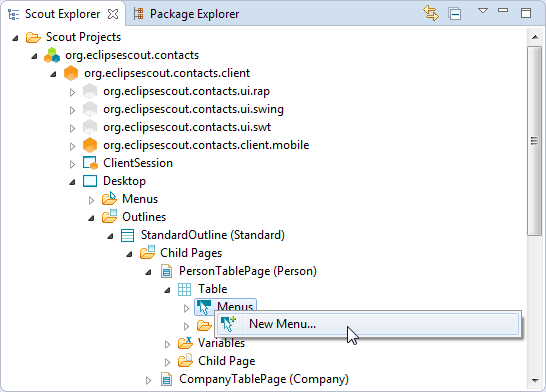
\includegraphics[width=7cm]{new_menu_editperson_contextmenu.png} \hspace{5mm}
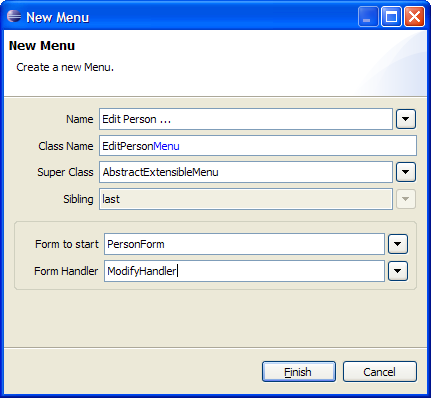
\includegraphics[width=7cm]{new_menu_editperson.png}
\caption{Add the Person edit menu to the person page.}
\figlabel{new_menu_editperson}
\end{figure}

Lorem ipsum will build an outline based Scout application featuring a navigation tree and pages to present information in tabular form. 
In addition, the application also shows how to work with menus and context menus, search forms, and forms to enter and/or update data. 
On the server side we show how to work with databases, how to use logging in Scout applications and how to lorem ipsum. 

\begin{figure}
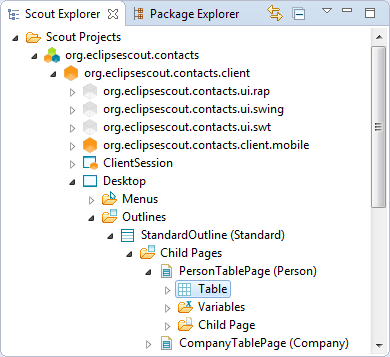
\includegraphics[width=7cm]{person_table_explorer.png} \hspace{5mm}
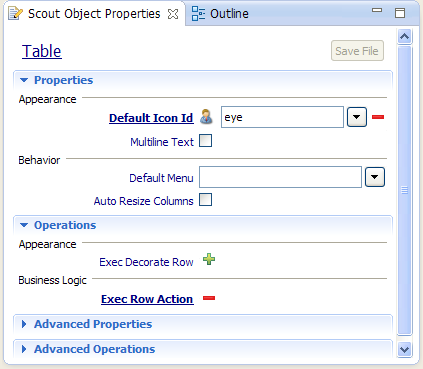
\includegraphics[width=7cm]{person_table_properties.png}
\caption{Set the behaviour for the row level action on the person table.}
\figlabel{person_table_properties}
\end{figure}

Lorem ipsum will build an outline based Scout application featuring a navigation tree and pages to present information in tabular form. 
In addition, the application also shows how to work with menus and context menus, search forms, and forms to enter and/or update data. 
On the server side we show how to work with databases, how to use logging in Scout applications and how to lorem ipsum. 

\begin{figure}
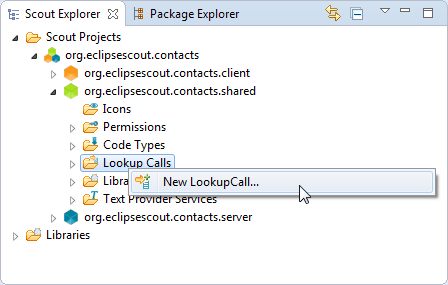
\includegraphics[width=7cm]{new_lookupcall_company_contextmenu.png} \hspace{2mm}
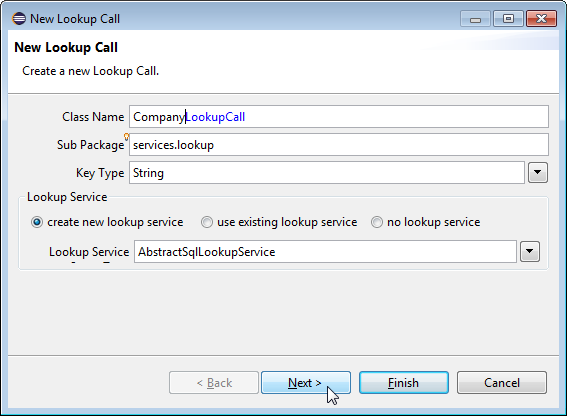
\includegraphics[width=7cm]{new_lookupcall_company_1.png} \hspace{2mm}
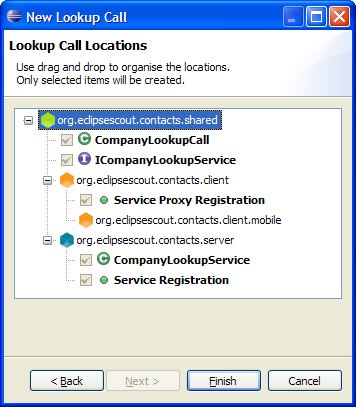
\includegraphics[width=7cm]{new_lookupcall_company_2.png}
\caption{Add the company lookup call to the applications shared node.}
\figlabel{new_lookupcall_company}
\end{figure}

Lorem ipsum will build an outline based Scout application featuring a navigation tree and pages to present information in tabular form. 
In addition, the application also shows how to work with menus and context menus, search forms, and forms to enter and/or update data. 
On the server side we show how to work with databases, how to use logging in Scout applications and how to lorem ipsum. 

\begin{figure}
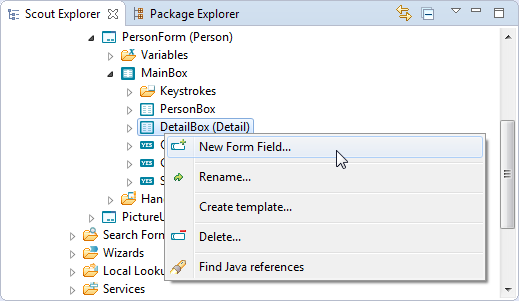
\includegraphics[width=7cm]{new_smartfield_company_contextmenu.png} \hspace{2mm}
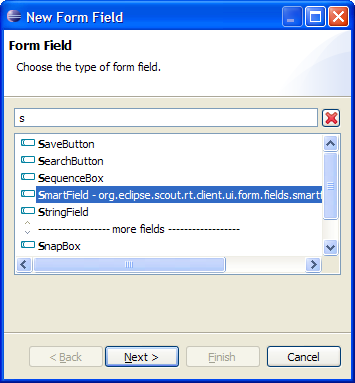
\includegraphics[width=7cm]{new_smartfield_company_1.png} \hspace{2mm}
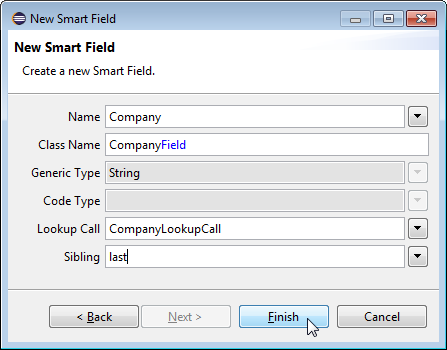
\includegraphics[width=7cm]{new_smartfield_company_2.png}
\caption{Add the company smartfield to the person form.}
\figlabel{new_smartfield_company}
\end{figure}

\begin{figure}
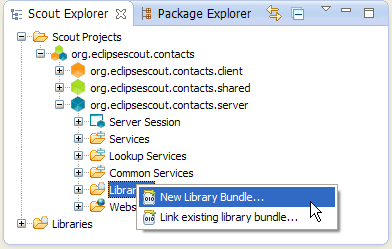
\includegraphics[width=7cm]{new_library_scribe_contextmenu.png} \hspace{5mm}
\caption{Add a new bundle to hold the Scribe JARs.}
\figlabel{new_library_scribe_contextmenu}
\end{figure}

Lorem ipsum will build an outline based Scout application featuring a navigation tree and pages to present information in tabular form. 
In addition, the application also shows how to work with menus and context menus, search forms, and forms to enter and/or update data. 
On the server side we show how to work with databases, how to use logging in Scout applications and how to lorem ipsum. 

\begin{figure}
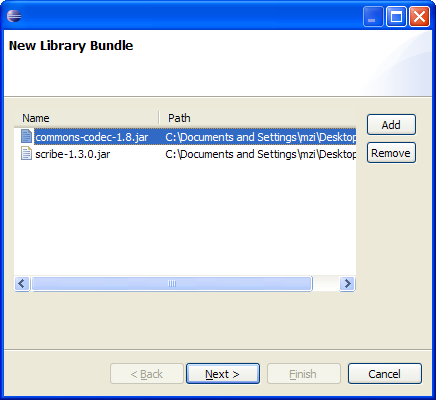
\includegraphics[width=7cm]{new_library_scribe_1.png} \hspace{5mm}
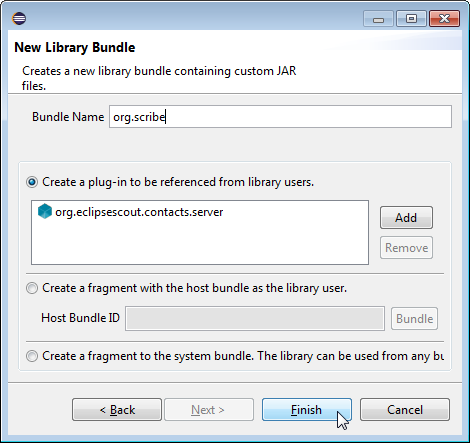
\includegraphics[width=7cm]{new_library_scribe_2.png}
\caption{Specify the JARs to be contained in the library bundle and the library name.}
\figlabel{new_library_scribe}
\end{figure}

Lorem ipsum will build an outline based Scout application featuring a navigation tree and pages to present information in tabular form. 
In addition, the application also shows how to work with menus and context menus, search forms, and forms to enter and/or update data. 
On the server side we show how to work with databases, how to use logging in Scout applications and how to lorem ipsum. 

\begin{figure}
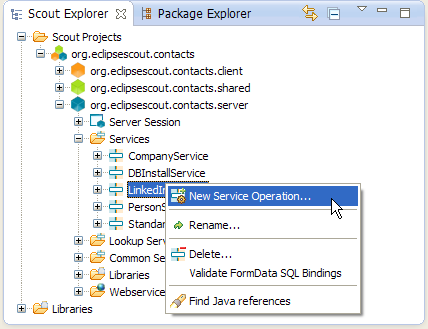
\includegraphics[width=7cm]{new_operation_authurl_contextmenu.png} \hspace{5mm}
\includegraphics[width=7cm]{new_operation_authurl.png}
\caption{Add the operation to retrieve an authentication URL.}
\figlabel{new_operation_authurl}
\end{figure}

Lorem ipsum will build an outline based Scout application featuring a navigation tree and pages to present information in tabular form. 
In addition, the application also shows how to work with menus and context menus, search forms, and forms to enter and/or update data. 
On the server side we show how to work with databases, how to use logging in Scout applications and how to lorem ipsum. 

\begin{figure}
\includegraphics[width=7cm]{new_operation_refreshtoken.png} \hspace{5mm}
\includegraphics[width=7cm]{new_operation_updatecontacts.png}
\caption{Add the operations to refresh the access token and to update the LinkedIn contacts.}
\figlabel{new_operation_refresh_update}
\end{figure}

Lorem ipsum will build an outline based Scout application featuring a navigation tree and pages to present information in tabular form. 
In addition, the application also shows how to work with menus and context menus, search forms, and forms to enter and/or update data. 
On the server side we show how to work with databases, how to use logging in Scout applications and how to lorem ipsum. 

\begin{figure}
\includegraphics[width=7cm]{new_form_token_1.png} \hspace{5mm}
\includegraphics[width=7cm]{new_form_token_2.png}
\caption{Add the form to refresh the LinkedIn access token.}
\figlabel{new_form_token}
\end{figure}

Lorem ipsum will build an outline based Scout application featuring a navigation tree and pages to present information in tabular form. 
In addition, the application also shows how to work with menus and context menus, search forms, and forms to enter and/or update data. 
On the server side we show how to work with databases, how to use logging in Scout applications and how to lorem ipsum. 

\begin{figure}
\includegraphics[width=7cm]{tokenform_securitycode_explorer.png} \hspace{5mm}
\includegraphics[width=7cm]{tokenform_securitycode_properties.png}
\caption{The token form in the explorer and the properties of the security code field.}
\figlabel{tokenform_securitycode}
\end{figure}

Lorem ipsum will build an outline based Scout application featuring a navigation tree and pages to present information in tabular form. 
In addition, the application also shows how to work with menus and context menus, search forms, and forms to enter and/or update data. 
On the server side we show how to work with databases, how to use logging in Scout applications and how to lorem ipsum. 

\begin{figure}
\includegraphics[width=7cm]{new_menu_refreshtoken_contextmenu.png} \hspace{5mm}
\includegraphics[width=7cm]{new_menu_refreshtoken.png}
\caption{Add the menu to open the LinkedIn token form.}
\figlabel{new_menu_refreshtoken}
\end{figure}

Lorem ipsum will build an outline based Scout application featuring a navigation tree and pages to present information in tabular form. 
In addition, the application also shows how to work with menus and context menus, search forms, and forms to enter and/or update data. 
On the server side we show how to work with databases, how to use logging in Scout applications and how to lorem ipsum. 

\begin{figure}
\includegraphics[width=7cm]{new_menu_updatecontacts_contextmenu.png} \hspace{5mm}
\includegraphics[width=7cm]{new_menu_updatecontacts.png}
\caption{Add the menu to update the LinkedIn contacts.}
\figlabel{new_menu_updatecontacts}
\end{figure}

server first, db setup service
server, derby sql service

server application

config.ini

\ifx\wholebook\relax\else
   \begin{thebibliography}{99}
  \addcontentsline{toc}{chapter}{Bibliography}
  
  % add/insert books in alphabetical order of 1st author
  
  \bibitem{batessierra05}
    \textit{Bert Bates, Kathy Sierra},
	\textbf{Head First Java} 2nd edition, 
	O'Reilly Media, 2005.

  \bibitem{bloch08} 
    \textit{Joshua Bloch},
    \textbf{Effective Java} 2nd edition, 
	Addison-Wesley, 2008.
	
  \bibitem{eckel06}
    \textit{Bruce Eckel},
	\textbf{Thinking in Java} 4th edition, 
	Prentice Hall International, 2006.

\end{thebibliography}

   \end{document}
\fi

% =========================================================================== %
